\documentclass[12pt,a4paper]{article}
\usepackage{tpl}
\dbeginn{10 ноября 2019 г.}{Команда, осень 2019}{Биекции и разбиения}{Петров Фёдор Алексеевич}

Будем смотреть на разные множества $\mathcal P_{\mathcal X}(n)$ --- разбиения $n=a_1+a_2+\ldots+a_k$, где $a_1\geq a_2\geq\ldots\geq a_k\in\mathbb N$ и $a_i$ обладают свойством $\mathcal X$. 

\theoremn{Эйлер} $|\mathcal P_{a_i=2r+1}(n)|=|\mathcal P_{a_i\neq a_j}(n)|$.\label{first}

\prooftms{first}
\prooftm{first} С одной стороны, $\mathcal P(n)=\bigcup\limits_{a=0}^n\mathcal P_{2r+1}(a)\times\mathcal P_{2r}(n-a)$. С другой стороны, пусть $n=a_1+a_2+\ldots+a_k$. Подчеркнём среди них те, которые встречаются нечётное количество раз. (например, в разбиении $14=3+3+3+2+2+1$ мы выделяем $3$ и $1$). Выделим их в множество $\mathcal P_{\neq}(a)$, а остальные разбить на пары, просуммировать и положить в $\mathcal P_{2r}(n-a)$. Таким образом, $|\mathcal P(n)|=\sum\limits_{a=0}^n|\mathcal P_{\neq}(a)|\cdot|\mathcal P_{2r}(n-a)|$. Индукция по $n$ заканчивает доказательство утверждения. \QEDA\\

\prooftmn{first}{Гляйшер} Пусть $n_i$ --- количество чисел, равных $i$, в разбиении на нечётные слагаемые. Запишем $n_i$ в двоичной системе и для каждого ненулевого слагаемого $2^r$ в разложении добавим в другое разбиение $2^r\cdot i$. На самом деле, это биекция (дальше мы её будем называть $\varphi_G$). \QEDA\\

\lemman{Гляйшер} Количество разбиений, в которых ровно $k$ чётных слагаемых, равно количеству разбиений, в которых повторяются ровно $k$.

\proof Произведём биекцию из <<$k$ чётных>> в <<$k$ повторяющихся>>. Поделим чётные пополам, а к остальным применим $\varphi_G$. Докажем, что это биекция. Пусть у нас есть $b_k$ слагаемых, равных $k$. Тогда если $b_k$ чётно, то превратим их в $\frac{b_k}{2}$ чисел, равных $2k$, иначе в $\frac{b_k-1}{2}$ слагаемых, равных $2k$, а последнее разделим на сколько-то максимальных одинаковых степеней двойки. \QEDA\\

\prooftmn{first}{Сильвестр} Рассмотрим какое-то разбиение и представим его в виде крюков, а затем разобьём их на строки и диагонали, например, $9+5+5+3$ превратится в $8+7+4+2+1$ следующим образом (и, оказывается, биективным):

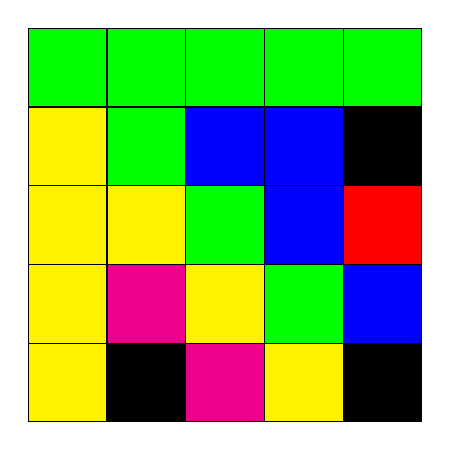
\begin{tikzpicture}
	\draw[fill=green] (0,4) -- (5,4) -- (5,5) -- (0,5) -- (0,4);
	\draw[fill=green] (1,4) -- (2,4) -- (2,3) -- (1,3);
	\draw[fill=green] (2,3) -- (3,3) -- (3,2) -- (2,2);
	\draw[fill=green] (3,2) -- (4,2) -- (4,1) -- (3,1);
	\draw[fill=black] (4,1) -- (5,1) -- (5,0) -- (4,0);
	\draw[fill=blue] (2,3) -- (2,4) -- (4,4) -- (4,3);
	\draw[fill=blue] (3,2) -- (3,3) -- (4,3) -- (4,2);
	\draw[fill=blue] (4,1) -- (4,2) -- (5,2) -- (5,1);
	\draw[fill=black] (4,4) -- (4,3) -- (5,3) -- (5,4);
	\draw[fill=red] (4,2) -- (4,3) -- (5,3) -- (5,2);
	\draw[fill=yellow] (0,0) -- (0,4) -- (1,4) -- (1,0);
	\draw[fill=yellow] (1,2) -- (1,3) -- (2,3) -- (2,2);
	\draw[fill=yellow] (2,1) -- (2,2) -- (3,2) -- (3,1);
	\draw[fill=yellow] (3,0) -- (3,1) -- (4,1) -- (4,0);
	\draw[fill=magenta] (1,1) -- (1,2) -- (2,2) -- (2,1);
	\draw[fill=magenta] (2,0) -- (2,1) -- (3,1) -- (3,0);
	\draw[fill=black] (1,0) -- (1,1) -- (2,1) -- (2,0);
	\draw[step=1,thin,black] (0,0) grid (5,5);
\end{tikzpicture}

Также эту биекцию можно сделать по другому. Представим разбиение в виде другой диаграммы Юнга и разобьём в крюки, как на рисунке ниже. Теперь $9+5+5+3=8+7+4+2+1$, потому что в 1-м крюке 8 элементов и 7 двоек, во втором 4 элемента и 2 двойки, в третьем 1 элемент и 0 двоек:

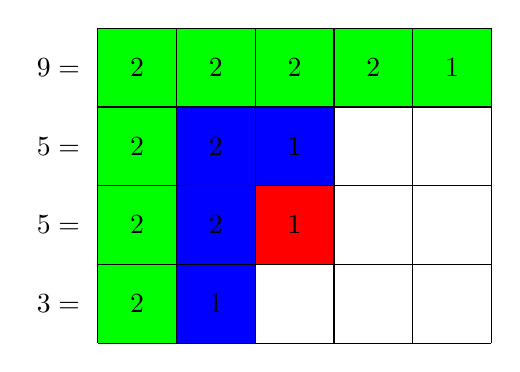
\begin{tikzpicture}
	\draw[fill=green] (0,-1) -- (0,3) -- (5,3) -- (5,2) -- (1,2) -- (1,-1) -- (0,-1);
	\draw[fill=blue] (1,-1) -- (1,2) -- (3,2) -- (3,1) -- (2,1) -- (2,-1) -- (1,-1);
	\draw[fill=red] (2,0) -- (2,1) -- (3,1) -- (3,0);
	\node at (0.5,2.5) {2};
	\node at (1.5,2.5) {2};
	\node at (2.5,2.5) {2};
	\node at (3.5,2.5) {2};
	\node at (4.5,2.5) {1};
	\node at (0.5,1.5) {2};
	\node at (1.5,1.5) {2};
	\node at (2.5,1.5) {1};
	\node at (0.5,0.5) {2};
	\node at (1.5,0.5) {2};
	\node at (2.5,0.5) {1};
	\node at (0.5,-0.5) {2};
	\node at (1.5,-0.5) {1};
	\node at (-0.5,-0.5) {$3=$};
	\node at (-0.5,0.5) {$5=$};
	\node at (-0.5,1.5) {$5=$};
	\node at (-0.5,2.5) {$9=$};
	\draw[step=1,thin,black] (0,-1) grid (5,3);
\end{tikzpicture}
\newpage

\prooftm{first} Воспользуемся производящими функциями. Производящая функция от $\mathcal P_{\neq}$ равна $(1+x)(1+x^2)\ldots$, а от $\mathcal P_{2r+1}$ --- \[
	\frac1{1-x}\cdot\frac1{1-x^3}\cdot\frac1{1-x^5}\cdot\ldots
.\] Видно, что они равны, например, можно воспользоваться формулой $1+x^k=\frac{1+x^{2k}}{1-x^k}$.\QEDA\\

\theoremn{Рамануджан} Количество разбиений на слагаемые, любые два из которых отличаются хотя бы на 2, равно количеству разбиений на слагаемые вида $5k\pm1$.\footnote{Для всех простых $p$ известны тождества подобного рода, где во второй штуке считаются разбиения с фиксированными остатками по модулю $p$.} \textit{Доказательство не рассказал, так как оно сложное.}\\

\theoremn{Эйлер} $(1-x)(1-x^2)(1-x^3)\ldots=1-x-x^2+x^5+x^7-x^{12}-\ldots=\sum\limits_{n=-\infty}^\infty (-1)^nx^{n(3n+1)/2}$.\label{pentagon}

\prooftms{pentagon}
\prooftm{pentagon} Посмотрим на бесконечный угол $45^\circ$. Пусть с вероятностью $1-x$ в каждой клетке угла вырастет кактус (кактусы в разных клетках независимо). Тогда $1-x^n$ --- вероятность того, что в $n$-м столбце вырастет кактус, а произведение слева $S$ --- вероятность того, что в каждом столбце вырастет кактус. Тогда $1-S$ --- вероятность того, что есть столбец без кактуса, и она равна \[
	x+x^2(T_{1,0}+T_{3,1}+T_{6,2}+\ldots)
,\] где $T_{r,s}$ --- вероятность того, что в $r$ клетках кактус есть, а в $s$ его нет. Обозначим эту сумму $T_{i,j}$ за $A$. Это вероятность такого события: возьмём горизонталь длиной (очень много), пусть первый кактус вырос в клетке номер $k$, тогда в каждом из различных множеств размером $2,3,\ldots,k$ есть кактус. Тогда $1-A$ --- это вероятность такого события: до появления первого кактуса в нижней строке есть строка целиком без кактусов. Посчитаем $1-A$: \[
1-A=x^3+x^5(T_{2,0}+T_{5,2}+T_{9,4}+\ldots)
.\] Обозначим сумму за $B$. Это то же самое, что и $A$, но высота строки увеличивается до 2, а каждое множество на 1. Таким образом можно получить такие равенства:
\begin{align*}
	1-S=x+x^2A;\\
	1-A=x^3+x^5B;\\
	1-B=x^5+x^8C;\\
	1-C=x^7+x^{11}D;\\
	\vdots
\end{align*} и если сложить эти равенства с коэффициентами $-x^2,x^7,-x^{15}$ и т.д., буквы $A,B,C$ и т.д. сократятся и получится искомое тождество.\QEDA\\

\prooftmn{pentagon}{Франклин} Легко видеть, что бесконечное произведение слева --- производящая функция от равенства количества разбиений на чётное количество различных слагаемое и на нечётное число различных слагаемых. Сделаем такое разбиение на пары $\varphi_F$. Пусть $a$ --- длина нижней строчки, $b$ --- длина диагонали, тогда если $a\leq b$, то увеличим первые $a$ строк и уберём $a$. Иначе уменьшим первые $b$ строк и добавим $b$. Тогда нам может не повезти в двух случаях:

\begin{enumerate}
	\item Пусть строки от $n$ до $2n-1$. Тогда мы не можем убрать нижнюю строку и увеличить первые $n$, потому что строк всего $n$. Это случай $\frac{n(3n-1)}{2}$.
\item Пусть строки от $n+1$ до $2n$. Тогда мы не можем убрать диагональ и поставить вниз, потому что она станет равна нижней строчке. Это случай $\frac{n(3n+1)}{2}$. \QEDA
\end{enumerate}\newpage

\lemman{Франклин} Разность количества разбиений числа $n>0$ на различные слагаемые (максимальное чётно) и количества разбиений на различные слагаемые (максимальное нечётно) равна
\begin{equation*}\begin{cases}
	+1,n=\frac{k(3k+1)}2,k\in\mathbb N;\\
	-1,n=\frac{k(3k-1)}2,k\in\mathbb N;\\
	0,\text{ иначе}.
\end{cases}\end{equation*}

\theoremn{Тройное тождество Якоби} \footnote{Это обобщение \ref{pentagon} после подстановки $z=x,q=x^3$.} \[
	\prod\limits_{n=1}^\infty (1-zq^{n-1})(1-z^{-1}q^n)(1-q^n)=\sum\limits_{k=-\infty} (-z)^kq^{k(k-1)/2}
.\]

\proof Обозначим $|\lambda|$ для разбиения $\lambda$ сумму его слагаемых. Заметим, что нам нужно доказать следующее: \[
	\prod\limits_{n=1}^\infty (1-zq^{n-1})(1-z^{-1}q^n)=\sum\limits_{k=-\infty} (-z)^kq^{k(k-1)/2}\cdot\sum\limits_\lambda x^\lambda
.\] Докажем, например, что коэффициент при $z^0$ такой же (для остальных идея та же самая, но надо будет пририсовывать треугольник слева). Возьмём разбиение числа и сделаем из него разбиение на $m$ положительных слагаемых и $m$ неотрицательных. Проведём диагональ и скажем, что всё, что ниже неё, одно разбиение, а то, что правее (и она сама), другое разбиение. \QEDA\\

\end{document}
